\documentclass[1p]{elsarticle_modified}
%\bibliographystyle{elsarticle-num}

%\usepackage[colorlinks]{hyperref}
%\usepackage{abbrmath_seonhwa} %\Abb, \Ascr, \Acal ,\Abf, \Afrak
\usepackage{amsfonts}
\usepackage{amssymb}
\usepackage{amsmath}
\usepackage{amsthm}
\usepackage{scalefnt}
\usepackage{amsbsy}
\usepackage{kotex}
\usepackage{caption}
\usepackage{subfig}
\usepackage{color}
\usepackage{graphicx}
\usepackage{xcolor} %% white, black, red, green, blue, cyan, magenta, yellow
\usepackage{float}
\usepackage{setspace}
\usepackage{hyperref}

\usepackage{tikz}
\usetikzlibrary{arrows}

\usepackage{multirow}
\usepackage{array} % fixed length table
\usepackage{hhline}

%%%%%%%%%%%%%%%%%%%%%
\makeatletter
\renewcommand*\env@matrix[1][\arraystretch]{%
	\edef\arraystretch{#1}%
	\hskip -\arraycolsep
	\let\@ifnextchar\new@ifnextchar
	\array{*\c@MaxMatrixCols c}}
\makeatother %https://tex.stackexchange.com/questions/14071/how-can-i-increase-the-line-spacing-in-a-matrix
%%%%%%%%%%%%%%%

\usepackage[normalem]{ulem}

\newcommand{\msout}[1]{\ifmmode\text{\sout{\ensuremath{#1}}}\else\sout{#1}\fi}
%SOURCE: \msout is \stkout macro in https://tex.stackexchange.com/questions/20609/strikeout-in-math-mode

\newcommand{\cancel}[1]{
	\ifmmode
	{\color{red}\msout{#1}}
	\else
	{\color{red}\sout{#1}}
	\fi
}

\newcommand{\add}[1]{
	{\color{blue}\uwave{#1}}
}

\newcommand{\replace}[2]{
	\ifmmode
	{\color{red}\msout{#1}}{\color{blue}\uwave{#2}}
	\else
	{\color{red}\sout{#1}}{\color{blue}\uwave{#2}}
	\fi
}

\newcommand{\Sol}{\mathcal{S}} %segment
\newcommand{\D}{D} %diagram
\newcommand{\A}{\mathcal{A}} %arc


%%%%%%%%%%%%%%%%%%%%%%%%%%%%%5 test

\def\sl{\operatorname{\textup{SL}}(2,\Cbb)}
\def\psl{\operatorname{\textup{PSL}}(2,\Cbb)}
\def\quan{\mkern 1mu \triangleright \mkern 1mu}

\theoremstyle{definition}
\newtheorem{thm}{Theorem}[section]
\newtheorem{prop}[thm]{Proposition}
\newtheorem{lem}[thm]{Lemma}
\newtheorem{ques}[thm]{Question}
\newtheorem{cor}[thm]{Corollary}
\newtheorem{defn}[thm]{Definition}
\newtheorem{exam}[thm]{Example}
\newtheorem{rmk}[thm]{Remark}
\newtheorem{alg}[thm]{Algorithm}

\newcommand{\I}{\sqrt{-1}}
\begin{document}

%\begin{frontmatter}
%
%\title{Boundary parabolic representations of knots up to 8 crossings}
%
%%% Group authors per affiliation:
%\author{Yunhi Cho} 
%\address{Department of Mathematics, University of Seoul, Seoul, Korea}
%\ead{yhcho@uos.ac.kr}
%
%
%\author{Seonhwa Kim} %\fnref{s_kim}}
%\address{Center for Geometry and Physics, Institute for Basic Science, Pohang, 37673, Korea}
%\ead{ryeona17@ibs.re.kr}
%
%\author{Hyuk Kim}
%\address{Department of Mathematical Sciences, Seoul National University, Seoul 08826, Korea}
%\ead{hyukkim@snu.ac.kr}
%
%\author{Seokbeom Yoon}
%\address{Department of Mathematical Sciences, Seoul National University, Seoul, 08826,  Korea}
%\ead{sbyoon15@snu.ac.kr}
%
%\begin{abstract}
%We find all boundary parabolic representation of knots up to 8 crossings.
%
%\end{abstract}
%\begin{keyword}
%    \MSC[2010] 57M25 
%\end{keyword}
%
%\end{frontmatter}

%\linenumbers
%\tableofcontents
%
\newcommand\colored[1]{\textcolor{white}{\rule[-0.35ex]{0.8em}{1.4ex}}\kern-0.8em\color{red} #1}%
%\newcommand\colored[1]{\textcolor{white}{ #1}\kern-2.17ex	\textcolor{white}{ #1}\kern-1.81ex	\textcolor{white}{ #1}\kern-2.15ex\color{red}#1	}

{\Large $\underline{9_{25}~(K9a_{4})}$}

\setlength{\tabcolsep}{10pt}
\renewcommand{\arraystretch}{1.6}
\vspace{1cm}\begin{tabular}{m{100pt}>{\centering\arraybackslash}m{274pt}}
\multirow{5}{120pt}{
	\centering
	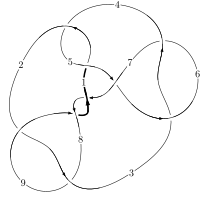
\includegraphics[width=112pt]{../../../GIT/diagram.site/Diagrams/png/60_9_25.png}\\
\ \ \ A knot diagram\footnotemark}&
\allowdisplaybreaks
\textbf{Linearized knot diagam} \\
\cline{2-2}
 &
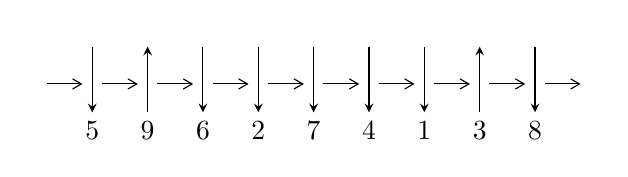
\begin{tikzpicture}[x=20pt, y=17pt]
	% nodes
	\node (C0) at (0, 0) {};
	\node (C1) at (1, 0) {};
	\node (C1U) at (1, +1) {};
	\node (C1D) at (1, -1) {5};

	\node (C2) at (2, 0) {};
	\node (C2U) at (2, +1) {};
	\node (C2D) at (2, -1) {9};

	\node (C3) at (3, 0) {};
	\node (C3U) at (3, +1) {};
	\node (C3D) at (3, -1) {6};

	\node (C4) at (4, 0) {};
	\node (C4U) at (4, +1) {};
	\node (C4D) at (4, -1) {2};

	\node (C5) at (5, 0) {};
	\node (C5U) at (5, +1) {};
	\node (C5D) at (5, -1) {7};

	\node (C6) at (6, 0) {};
	\node (C6U) at (6, +1) {};
	\node (C6D) at (6, -1) {4};

	\node (C7) at (7, 0) {};
	\node (C7U) at (7, +1) {};
	\node (C7D) at (7, -1) {1};

	\node (C8) at (8, 0) {};
	\node (C8U) at (8, +1) {};
	\node (C8D) at (8, -1) {3};

	\node (C9) at (9, 0) {};
	\node (C9U) at (9, +1) {};
	\node (C9D) at (9, -1) {8};
	\node (C10) at (10, 0) {};

	% arrows
	\draw[->,>={angle 60}]
	(C0) edge (C1) (C1) edge (C2) (C2) edge (C3) (C3) edge (C4) (C4) edge (C5) (C5) edge (C6) (C6) edge (C7) (C7) edge (C8) (C8) edge (C9) (C9) edge (C10) ;	\draw[->,>=stealth]
	(C1U) edge (C1D) (C2D) edge (C2U) (C3U) edge (C3D) (C4U) edge (C4D) (C5U) edge (C5D) (C6U) edge (C6D) (C7U) edge (C7D) (C8D) edge (C8U) (C9U) edge (C9D) ;
	\end{tikzpicture} \\
\hhline{~~} \\& 
\textbf{Solving Sequence} \\ \cline{2-2} 
 &
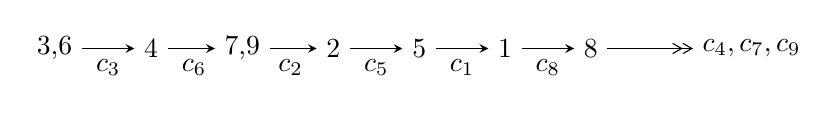
\begin{tikzpicture}[x=31pt, y=7pt]
	% node
	\node (A0) at (-1/8, 0) {3,6};
	\node (A1) at (1, 0) {4};
	\node (A2) at (33/16, 0) {7,9};
	\node (A3) at (25/8, 0) {2};
	\node (A4) at (33/8, 0) {5};
	\node (A5) at (41/8, 0) {1};
	\node (A6) at (49/8, 0) {8};
	\node (C1) at (1/2, -1) {$c_{3}$};
	\node (C2) at (3/2, -1) {$c_{6}$};
	\node (C3) at (21/8, -1) {$c_{2}$};
	\node (C4) at (29/8, -1) {$c_{5}$};
	\node (C5) at (37/8, -1) {$c_{1}$};
	\node (C6) at (45/8, -1) {$c_{8}$};
	\node (A7) at (8, 0) {$c_{4},c_{7},c_{9}$};

	% edge
	\draw[->,>=stealth]	
	(A0) edge (A1) (A1) edge (A2) (A2) edge (A3) (A3) edge (A4) (A4) edge (A5) (A5) edge (A6) ;
	\draw[->>,>={angle 60}]	
	(A6) edge (A7);
\end{tikzpicture} \\ 

\end{tabular} \\

\footnotetext{
The image of knot diagram is generated by the software ``\textbf{Draw programme}" developed by Andrew Bartholomew(\url{http://www.layer8.co.uk/maths/draw/index.htm\#Running-draw}), where we modified some parts for our purpose(\url{https://github.com/CATsTAILs/LinksPainter}).
}\phantom \\ \newline 
\centering \textbf{Ideals for irreducible components\footnotemark of $X_{\text{par}}$} 
 
\begin{align*}
I^u_{1}&=\langle 
- u^{24}-2 u^{23}+\cdots+2 b+1,\;- u^{24}-2 u^{23}+\cdots+a+5 u,\;u^{25}+3 u^{24}+\cdots-4 u-1\rangle \\
I^u_{2}&=\langle 
2 b- a-1,\;a^2+3,\;u-1\rangle \\
\\
\end{align*}
\raggedright * 2 irreducible components of $\dim_{\mathbb{C}}=0$, with total 27 representations.\\
\footnotetext{All coefficients of polynomials are rational numbers. But the coefficients are sometimes approximated in decimal forms when there is not enough margin.}
\newpage
\renewcommand{\arraystretch}{1}
\centering \section*{I. $I^u_{1}= \langle - u^{24}-2 u^{23}+\cdots+2 b+1,\;- u^{24}-2 u^{23}+\cdots+a+5 u,\;u^{25}+3 u^{24}+\cdots-4 u-1 \rangle$}
\flushleft \textbf{(i) Arc colorings}\\
\begin{tabular}{m{7pt} m{180pt} m{7pt} m{180pt} }
\flushright $a_{3}=$&$\begin{pmatrix}1\\0\end{pmatrix}$ \\
\flushright $a_{6}=$&$\begin{pmatrix}0\\u\end{pmatrix}$ \\
\flushright $a_{4}=$&$\begin{pmatrix}1\\u^2\end{pmatrix}$ \\
\flushright $a_{7}=$&$\begin{pmatrix}- u\\- u^3+u\end{pmatrix}$ \\
\flushright $a_{9}=$&$\begin{pmatrix}u^{24}+2 u^{23}+\cdots-5 u^2-5 u\\\frac{1}{2} u^{24}+u^{23}+\cdots-\frac{7}{2} u-\frac{1}{2}\end{pmatrix}$ \\
\flushright $a_{2}=$&$\begin{pmatrix}\frac{7}{2} u^{24}+9 u^{23}+\cdots-\frac{33}{2} u-\frac{9}{2}\\\frac{3}{2} u^{24}+4 u^{23}+\cdots-\frac{13}{2} u-\frac{5}{2}\end{pmatrix}$ \\
\flushright $a_{5}=$&$\begin{pmatrix}u^3\\u^5- u^3+u\end{pmatrix}$ \\
\flushright $a_{1}=$&$\begin{pmatrix}\frac{3}{2} u^{24}+3 u^{23}+\cdots-\frac{15}{2} u-\frac{3}{2}\\\frac{5}{2} u^{24}+6 u^{23}+\cdots-\frac{21}{2} u-\frac{7}{2}\end{pmatrix}$ \\
\flushright $a_{8}=$&$\begin{pmatrix}\frac{1}{2} u^{24}+u^{23}+\cdots-\frac{3}{2} u+\frac{1}{2}\\\frac{1}{2} u^{24}+u^{23}+\cdots-\frac{7}{2} u-\frac{1}{2}\end{pmatrix}$\\ \flushright $a_{8}=$&$\begin{pmatrix}\frac{1}{2} u^{24}+u^{23}+\cdots-\frac{3}{2} u+\frac{1}{2}\\\frac{1}{2} u^{24}+u^{23}+\cdots-\frac{7}{2} u-\frac{1}{2}\end{pmatrix}$\\&\end{tabular}
\flushleft \textbf{(ii) Obstruction class $= -1$}\\~\\
\flushleft \textbf{(iii) Cusp Shapes $= 2 u^{24}+7 u^{23}-5 u^{22}-42 u^{21}-25 u^{20}+108 u^{19}+144 u^{18}-128 u^{17}-357 u^{16}+2 u^{15}+526 u^{14}+286 u^{13}-498 u^{12}-538 u^{11}+238 u^{10}+584 u^9+35 u^8-389 u^7-165 u^6+164 u^5+119 u^4-22 u^3-38 u^2-6 u-5$}\\~\\
\newpage\renewcommand{\arraystretch}{1}
\flushleft \textbf{(iv) u-Polynomials at the component}\newline \\
\begin{tabular}{m{50pt}|m{274pt}}
Crossings & \hspace{64pt}u-Polynomials at each crossing \\
\hline $$\begin{aligned}c_{1},c_{4}\end{aligned}$$&$\begin{aligned}
&u^{25}- u^{24}+\cdots+4 u+4
\end{aligned}$\\
\hline $$\begin{aligned}c_{2},c_{8}\end{aligned}$$&$\begin{aligned}
&u^{25}+2 u^{24}+\cdots+3 u+1
\end{aligned}$\\
\hline $$\begin{aligned}c_{3},c_{6}\end{aligned}$$&$\begin{aligned}
&u^{25}-3 u^{24}+\cdots-4 u+1
\end{aligned}$\\
\hline $$\begin{aligned}c_{5}\end{aligned}$$&$\begin{aligned}
&u^{25}+11 u^{24}+\cdots-2 u+1
\end{aligned}$\\
\hline $$\begin{aligned}c_{7},c_{9}\end{aligned}$$&$\begin{aligned}
&u^{25}+8 u^{24}+\cdots+11 u-1
\end{aligned}$\\
\hline
\end{tabular}\\~\\
\newpage\renewcommand{\arraystretch}{1}
\flushleft \textbf{(v) Riley Polynomials at the component}\newline \\
\begin{tabular}{m{50pt}|m{274pt}}
Crossings & \hspace{64pt}Riley Polynomials at each crossing \\
\hline $$\begin{aligned}c_{1},c_{4}\end{aligned}$$&$\begin{aligned}
&y^{25}+15 y^{24}+\cdots-88 y-16
\end{aligned}$\\
\hline $$\begin{aligned}c_{2},c_{8}\end{aligned}$$&$\begin{aligned}
&y^{25}+8 y^{24}+\cdots+11 y-1
\end{aligned}$\\
\hline $$\begin{aligned}c_{3},c_{6}\end{aligned}$$&$\begin{aligned}
&y^{25}-11 y^{24}+\cdots-2 y-1
\end{aligned}$\\
\hline $$\begin{aligned}c_{5}\end{aligned}$$&$\begin{aligned}
&y^{25}+9 y^{24}+\cdots-2 y-1
\end{aligned}$\\
\hline $$\begin{aligned}c_{7},c_{9}\end{aligned}$$&$\begin{aligned}
&y^{25}+20 y^{24}+\cdots+251 y-1
\end{aligned}$\\
\hline
\end{tabular}\\~\\
\newpage\flushleft \textbf{(vi) Complex Volumes and Cusp Shapes}
$$\begin{array}{c|c|c}  
\text{Solutions to }I^u_{1}& \I (\text{vol} + \sqrt{-1}CS) & \text{Cusp shape}\\
 \hline 
\begin{aligned}
u &= \phantom{-}0.781818 + 0.585895 I \\
a &= -0.235890 - 0.629868 I \\
b &= \phantom{-}0.734813 + 0.804167 I\end{aligned}
 & \phantom{-}1.52493 + 0.43356 I & -3.08804 + 0.04506 I \\ \hline\begin{aligned}
u &= \phantom{-}0.781818 - 0.585895 I \\
a &= -0.235890 + 0.629868 I \\
b &= \phantom{-}0.734813 - 0.804167 I\end{aligned}
 & \phantom{-}1.52493 - 0.43356 I & -3.08804 - 0.04506 I \\ \hline\begin{aligned}
u &= -0.840318 + 0.621070 I \\
a &= \phantom{-}0.114344 + 0.489930 I \\
b &= \phantom{-}0.723797 + 0.117969 I\end{aligned}
 & \phantom{-}2.10182 + 2.44039 I & -0.16599 - 3.61173 I \\ \hline\begin{aligned}
u &= -0.840318 - 0.621070 I \\
a &= \phantom{-}0.114344 - 0.489930 I \\
b &= \phantom{-}0.723797 - 0.117969 I\end{aligned}
 & \phantom{-}2.10182 - 2.44039 I & -0.16599 + 3.61173 I \\ \hline\begin{aligned}
u &= -0.479273 + 0.936834 I \\
a &= \phantom{-}0.544317 + 0.502084 I \\
b &= -0.776571 + 0.974090 I\end{aligned}
 & \phantom{-}6.34798 - 5.44271 I & -0.49829 + 3.51350 I \\ \hline\begin{aligned}
u &= -0.479273 - 0.936834 I \\
a &= \phantom{-}0.544317 - 0.502084 I \\
b &= -0.776571 - 0.974090 I\end{aligned}
 & \phantom{-}6.34798 + 5.44271 I & -0.49829 - 3.51350 I \\ \hline\begin{aligned}
u &= -0.563663 + 0.911236 I \\
a &= \phantom{-}0.646213 - 0.436873 I \\
b &= -0.842489 - 0.787076 I\end{aligned}
 & \phantom{-}6.92874 + 0.59688 I & \phantom{-}0.46758 - 1.80507 I \\ \hline\begin{aligned}
u &= -0.563663 - 0.911236 I \\
a &= \phantom{-}0.646213 + 0.436873 I \\
b &= -0.842489 + 0.787076 I\end{aligned}
 & \phantom{-}6.92874 - 0.59688 I & \phantom{-}0.46758 + 1.80507 I \\ \hline\begin{aligned}
u &= \phantom{-}0.903290 + 0.591334 I \\
a &= -1.72740 - 1.15219 I \\
b &= \phantom{-}0.719637 - 0.929655 I\end{aligned}
 & \phantom{-}1.14086 - 5.11531 I & -4.18255 + 5.48464 I \\ \hline\begin{aligned}
u &= \phantom{-}0.903290 - 0.591334 I \\
a &= -1.72740 + 1.15219 I \\
b &= \phantom{-}0.719637 + 0.929655 I\end{aligned}
 & \phantom{-}1.14086 + 5.11531 I & -4.18255 - 5.48464 I\\
 \hline 
 \end{array}$$\newpage$$\begin{array}{c|c|c}  
\text{Solutions to }I^u_{1}& \I (\text{vol} + \sqrt{-1}CS) & \text{Cusp shape}\\
 \hline 
\begin{aligned}
u &= \phantom{-}1.073950 + 0.294320 I \\
a &= \phantom{-}1.15104 + 1.96262 I \\
b &= -0.071208 + 0.875733 I\end{aligned}
 & -3.46537 - 1.05922 I & -11.39395 + 0.37058 I \\ \hline\begin{aligned}
u &= \phantom{-}1.073950 - 0.294320 I \\
a &= \phantom{-}1.15104 - 1.96262 I \\
b &= -0.071208 - 0.875733 I\end{aligned}
 & -3.46537 + 1.05922 I & -11.39395 - 0.37058 I \\ \hline\begin{aligned}
u &= -1.012760 + 0.537221 I \\
a &= -0.77689 + 2.25052 I \\
b &= \phantom{-}0.204213 + 1.096690 I\end{aligned}
 & -1.91594 + 5.41987 I & -7.35697 - 6.54919 I \\ \hline\begin{aligned}
u &= -1.012760 - 0.537221 I \\
a &= -0.77689 - 2.25052 I \\
b &= \phantom{-}0.204213 - 1.096690 I\end{aligned}
 & -1.91594 - 5.41987 I & -7.35697 + 6.54919 I \\ \hline\begin{aligned}
u &= \phantom{-}0.819709\phantom{ +0.000000I} \\
a &= \phantom{-}0.530934\phantom{ +0.000000I} \\
b &= -0.251925\phantom{ +0.000000I}\end{aligned}
 & -1.19408\phantom{ +0.000000I} & -8.44380\phantom{ +0.000000I} \\ \hline\begin{aligned}
u &= -0.706780 + 0.369020 I \\
a &= \phantom{-}0.42079 - 1.91115 I \\
b &= \phantom{-}0.427994 - 1.010940 I\end{aligned}
 & -0.62342 - 1.39976 I & -3.04278 + 0.06062 I \\ \hline\begin{aligned}
u &= -0.706780 - 0.369020 I \\
a &= \phantom{-}0.42079 + 1.91115 I \\
b &= \phantom{-}0.427994 + 1.010940 I\end{aligned}
 & -0.62342 + 1.39976 I & -3.04278 - 0.06062 I \\ \hline\begin{aligned}
u &= -1.089150 + 0.711472 I \\
a &= -0.490999 - 0.203095 I \\
b &= -0.865451 + 0.706038 I\end{aligned}
 & \phantom{-}5.32382 + 5.36637 I & -1.53322 - 3.05337 I \\ \hline\begin{aligned}
u &= -1.089150 - 0.711472 I \\
a &= -0.490999 + 0.203095 I \\
b &= -0.865451 - 0.706038 I\end{aligned}
 & \phantom{-}5.32382 - 5.36637 I & -1.53322 + 3.05337 I \\ \hline\begin{aligned}
u &= \phantom{-}1.306760 + 0.052319 I \\
a &= -0.27343 - 1.51011 I \\
b &= -0.691717 - 0.872891 I\end{aligned}
 & -0.20167 + 2.66172 I & -2.71477 - 3.57661 I\\
 \hline 
 \end{array}$$\newpage$$\begin{array}{c|c|c}  
\text{Solutions to }I^u_{1}& \I (\text{vol} + \sqrt{-1}CS) & \text{Cusp shape}\\
 \hline 
\begin{aligned}
u &= \phantom{-}1.306760 - 0.052319 I \\
a &= -0.27343 + 1.51011 I \\
b &= -0.691717 + 0.872891 I\end{aligned}
 & -0.20167 - 2.66172 I & -2.71477 + 3.57661 I \\ \hline\begin{aligned}
u &= -1.139240 + 0.687767 I \\
a &= \phantom{-}1.14519 - 1.80727 I \\
b &= -0.753308 - 1.027550 I\end{aligned}
 & \phantom{-}4.33274 + 11.39030 I & -3.28983 - 7.76664 I \\ \hline\begin{aligned}
u &= -1.139240 - 0.687767 I \\
a &= \phantom{-}1.14519 + 1.80727 I \\
b &= -0.753308 + 1.027550 I\end{aligned}
 & \phantom{-}4.33274 - 11.39030 I & -3.28983 + 7.76664 I \\ \hline\begin{aligned}
u &= -0.144497 + 0.357570 I \\
a &= \phantom{-}1.21724 - 0.74670 I \\
b &= \phantom{-}0.316251 - 0.806276 I\end{aligned}
 & -0.33578 - 1.50728 I & -2.97928 + 4.31266 I \\ \hline\begin{aligned}
u &= -0.144497 - 0.357570 I \\
a &= \phantom{-}1.21724 + 0.74670 I \\
b &= \phantom{-}0.316251 + 0.806276 I\end{aligned}
 & -0.33578 + 1.50728 I & -2.97928 - 4.31266 I\\
 \hline 
 \end{array}$$\newpage\newpage\renewcommand{\arraystretch}{1}
\centering \section*{II. $I^u_{2}= \langle 2 b- a-1,\;a^2+3,\;u-1 \rangle$}
\flushleft \textbf{(i) Arc colorings}\\
\begin{tabular}{m{7pt} m{180pt} m{7pt} m{180pt} }
\flushright $a_{3}=$&$\begin{pmatrix}1\\0\end{pmatrix}$ \\
\flushright $a_{6}=$&$\begin{pmatrix}0\\1\end{pmatrix}$ \\
\flushright $a_{4}=$&$\begin{pmatrix}1\\1\end{pmatrix}$ \\
\flushright $a_{7}=$&$\begin{pmatrix}-1\\0\end{pmatrix}$ \\
\flushright $a_{9}=$&$\begin{pmatrix}a\\\frac{1}{2} a+\frac{1}{2}\end{pmatrix}$ \\
\flushright $a_{2}=$&$\begin{pmatrix}\frac{1}{2} a-\frac{1}{2}\\\frac{1}{2} a-\frac{1}{2}\end{pmatrix}$ \\
\flushright $a_{5}=$&$\begin{pmatrix}1\\1\end{pmatrix}$ \\
\flushright $a_{1}=$&$\begin{pmatrix}\frac{1}{2} a-\frac{1}{2}\\\frac{1}{2} a-\frac{1}{2}\end{pmatrix}$ \\
\flushright $a_{8}=$&$\begin{pmatrix}\frac{1}{2} a-\frac{1}{2}\\\frac{1}{2} a+\frac{1}{2}\end{pmatrix}$\\ \flushright $a_{8}=$&$\begin{pmatrix}\frac{1}{2} a-\frac{1}{2}\\\frac{1}{2} a+\frac{1}{2}\end{pmatrix}$\\&\end{tabular}
\flushleft \textbf{(ii) Obstruction class $= 1$}\\~\\
\flushleft \textbf{(iii) Cusp Shapes $= -2 a-9$}\\~\\
\newpage\renewcommand{\arraystretch}{1}
\flushleft \textbf{(iv) u-Polynomials at the component}\newline \\
\begin{tabular}{m{50pt}|m{274pt}}
Crossings & \hspace{64pt}u-Polynomials at each crossing \\
\hline $$\begin{aligned}c_{1},c_{4}\end{aligned}$$&$\begin{aligned}
&u^2
\end{aligned}$\\
\hline $$\begin{aligned}c_{2},c_{7}\end{aligned}$$&$\begin{aligned}
&u^2- u+1
\end{aligned}$\\
\hline $$\begin{aligned}c_{3},c_{5}\end{aligned}$$&$\begin{aligned}
&(u-1)^2
\end{aligned}$\\
\hline $$\begin{aligned}c_{6}\end{aligned}$$&$\begin{aligned}
&(u+1)^2
\end{aligned}$\\
\hline $$\begin{aligned}c_{8},c_{9}\end{aligned}$$&$\begin{aligned}
&u^2+u+1
\end{aligned}$\\
\hline
\end{tabular}\\~\\
\newpage\renewcommand{\arraystretch}{1}
\flushleft \textbf{(v) Riley Polynomials at the component}\newline \\
\begin{tabular}{m{50pt}|m{274pt}}
Crossings & \hspace{64pt}Riley Polynomials at each crossing \\
\hline $$\begin{aligned}c_{1},c_{4}\end{aligned}$$&$\begin{aligned}
&y^2
\end{aligned}$\\
\hline $$\begin{aligned}c_{2},c_{7},c_{8}\\c_{9}\end{aligned}$$&$\begin{aligned}
&y^2+y+1
\end{aligned}$\\
\hline $$\begin{aligned}c_{3},c_{5},c_{6}\end{aligned}$$&$\begin{aligned}
&(y-1)^2
\end{aligned}$\\
\hline
\end{tabular}\\~\\
\newpage\flushleft \textbf{(vi) Complex Volumes and Cusp Shapes}
$$\begin{array}{c|c|c}  
\text{Solutions to }I^u_{2}& \I (\text{vol} + \sqrt{-1}CS) & \text{Cusp shape}\\
 \hline 
\begin{aligned}
u &= \phantom{-}1.00000\phantom{ +0.000000I} \\
a &= \phantom{-0.000000 -}1.73205 I \\
b &= \phantom{-}0.500000 + 0.866025 I\end{aligned}
 & -1.64493 + 2.02988 I & -9.00000 - 3.46410 I \\ \hline\begin{aligned}
u &= \phantom{-}1.00000\phantom{ +0.000000I} \\
a &= \phantom{-0.000000 } -1.73205 I \\
b &= \phantom{-}0.500000 - 0.866025 I\end{aligned}
 & -1.64493 - 2.02988 I & -9.00000 + 3.46410 I\\
 \hline 
 \end{array}$$\newpage
\newpage\renewcommand{\arraystretch}{1}
\centering \section*{ III. u-Polynomials}
\begin{tabular}{m{50pt}|m{274pt}}
Crossings & \hspace{64pt}u-Polynomials at each crossing \\
\hline $$\begin{aligned}c_{1},c_{4}\end{aligned}$$&$\begin{aligned}
&u^2(u^{25}- u^{24}+\cdots+4 u+4)
\end{aligned}$\\
\hline $$\begin{aligned}c_{2}\end{aligned}$$&$\begin{aligned}
&(u^2- u+1)(u^{25}+2 u^{24}+\cdots+3 u+1)
\end{aligned}$\\
\hline $$\begin{aligned}c_{3}\end{aligned}$$&$\begin{aligned}
&((u-1)^2)(u^{25}-3 u^{24}+\cdots-4 u+1)
\end{aligned}$\\
\hline $$\begin{aligned}c_{5}\end{aligned}$$&$\begin{aligned}
&((u-1)^2)(u^{25}+11 u^{24}+\cdots-2 u+1)
\end{aligned}$\\
\hline $$\begin{aligned}c_{6}\end{aligned}$$&$\begin{aligned}
&((u+1)^2)(u^{25}-3 u^{24}+\cdots-4 u+1)
\end{aligned}$\\
\hline $$\begin{aligned}c_{7}\end{aligned}$$&$\begin{aligned}
&(u^2- u+1)(u^{25}+8 u^{24}+\cdots+11 u-1)
\end{aligned}$\\
\hline $$\begin{aligned}c_{8}\end{aligned}$$&$\begin{aligned}
&(u^2+u+1)(u^{25}+2 u^{24}+\cdots+3 u+1)
\end{aligned}$\\
\hline $$\begin{aligned}c_{9}\end{aligned}$$&$\begin{aligned}
&(u^2+u+1)(u^{25}+8 u^{24}+\cdots+11 u-1)
\end{aligned}$\\
\hline
\end{tabular}\newpage\renewcommand{\arraystretch}{1}
\centering \section*{ IV. Riley Polynomials}
\begin{tabular}{m{50pt}|m{274pt}}
Crossings & \hspace{64pt}Riley Polynomials at each crossing \\
\hline $$\begin{aligned}c_{1},c_{4}\end{aligned}$$&$\begin{aligned}
&y^2(y^{25}+15 y^{24}+\cdots-88 y-16)
\end{aligned}$\\
\hline $$\begin{aligned}c_{2},c_{8}\end{aligned}$$&$\begin{aligned}
&(y^2+y+1)(y^{25}+8 y^{24}+\cdots+11 y-1)
\end{aligned}$\\
\hline $$\begin{aligned}c_{3},c_{6}\end{aligned}$$&$\begin{aligned}
&((y-1)^2)(y^{25}-11 y^{24}+\cdots-2 y-1)
\end{aligned}$\\
\hline $$\begin{aligned}c_{5}\end{aligned}$$&$\begin{aligned}
&((y-1)^2)(y^{25}+9 y^{24}+\cdots-2 y-1)
\end{aligned}$\\
\hline $$\begin{aligned}c_{7},c_{9}\end{aligned}$$&$\begin{aligned}
&(y^2+y+1)(y^{25}+20 y^{24}+\cdots+251 y-1)
\end{aligned}$\\
\hline
\end{tabular}
\vskip 2pc
\end{document}